%------------------------------------------------------------%

\chapter{Metodologia}
\label{cap:trabalhos:metodologia}

Este capítulo apresenta a metodologia adotada para o desenvolvimento e validação do sistema proposto neste trabalho. O estudo foi estruturado em duas etapas principais: simulação e implementação real. A simulação foi realizada utilizando o ambiente CoppeliaSim integrado ao Robot Operating System (ROS), permitindo a criação de cenários controlados para a coleta inicial de dados e testes com diferentes configurações robóticas. Na etapa real, os dados foram coletados em um ambiente físico montado no laboratório, onde o sistema foi submetido a condições práticas semelhantes às encontradas em linhas de transmissão reais. Além disso, são descritos os processos de aquisição, armazenamento e pré-processamento dos dados provenientes de sensores LiDAR e câmera de profundidade, bem como a construção das cenas simuladas e físicas, os modelos e algoritmos de aprendizado de máquina utilizados no treinamento e avaliação do sistema. Essa abordagem híbrida entre simulação e experimentação física visa garantir robustez, reprodutibilidade e aplicabilidade prática dos resultados obtidos ao longo do projeto.

\section{Ambiente de Desenvolvimento e Simulação}

Nesta seção, são descritas as ferramentas e tecnologias utilizadas para a construção do ambiente de simulação e desenvolvimento do projeto. O foco está na criação de uma infraestrutura que permita tanto a comunicação entre sensores e o robô quanto a simulação realista das operações. A subseção está dividida em quatro partes: introdução ao ROS (Robot Operating System), introdução ao CoppeliaSim, comunicação entre componentes e justificativa do uso de um ambiente híbrido.


\subsection{Robot Operating System}

O \textit{Robot Operating System} é um middleware de código aberto amplamente utilizado no desenvolvimento de sistemas robóticos. Longe de ser um sistema operacional tradicional, o ROS funciona como uma camada de abstração que oferece um conjunto de bibliotecas e ferramentas para simplificar a criação de softwares robóticos complexos. Ele fornece funcionalidades essenciais como gerenciamento de pacotes, comunicação entre processos (nós), manipulação de sensores e atuadores, visualização de dados e integração com ambientes de simulação \cite{quigley2009ros}. Neste projeto foi adotada a distribuição \textbf{ROS Noetic Ninjemys}, que é a última versão de longo suporte (LTS) da linha ROS 1 e é compatível com o sistema operacional \textbf{Ubuntu 20.04}. A necessidade de uma versão específica do sistema operacional se dá pelo fato de que o ROS é altamente dependente do ambiente Linux e das versões específicas das bibliotecas de sistema, que variam entre distribuições e versões do Ubuntu. Isso garante estabilidade e compatibilidade com os pacotes oficiais mantidos pela comunidade. A escolha do ROS Noetic também se justifica pelo alinhamento com as plataformas robóticas consideradas no projeto, as quais já utilizam o ROS como base para controle de seus elementos, permitindo uma integração mais fluida e reduzindo o esforço de configuração e implementação de funcionalidades. Além disso, o ecossistema do ROS conta com uma vasta gama de bibliotecas e drivers desenvolvidos e mantidos pela comunidade, oferecendo suporte a diversos sensores, como o LiDAR (Light Detection and Ranging) e câmeras de profundidade, utilizados neste trabalho. Essa modularidade e flexibilidade tornam-o uma escolha ideal para o desenvolvimento de aplicações autônomas e simulações realistas em ambientes robóticos.

No ROS, a arquitetura é baseada em uma estrutura distribuída composta por nós (\textit{nodes}) que se comunicam entre si por meio de tópicos (\textit{topics}). Cada nó pode atuar como publicador (\textit{publisher}) ou assinante (\textit{subscriber}), permitindo a troca de mensagens de forma assíncrona. Essa estrutura possibilita uma comunicação modular e flexível entre diferentes componentes do sistema robótico. No contexto deste projeto, foram definidos nós específicos para realizar o controle, aquisição, armazenamento e simulação dos dados. Um dos tópicos foi dedicado à configuração dos sensores, no qual os próprios sensores atuam como assinantes e recebem parâmetros de operação — como limites de leitura e frequência de varredura — a partir de um nó publicador controlado pelo usuário. Paralelamente, os sensores também atuam como publicadores em seus respectivos tópicos de dados, transmitindo continuamente as informações captadas. Esses tópicos são monitorados por nós assinantes responsáveis por armazenar os dados em arquivos locais, para posterior análise e uso no treinamento dos modelos de classificação. Essa organização garante a separação de responsabilidades e facilita a manutenção e expansão do sistema.

\subsubsection{Ferramentas do ROS}

O funcionamento do ROS depende da execução do \textit{roscore}, um serviço mestre responsável por gerenciar a comunicação entre os nós. O \textit{roscore} atua como um servidor central que permite o registro e a descoberta de nós, tópicos e serviços, garantindo que os nós publicadores e assinantes consigam localizar-se mutuamente em tempo de execução. Após sua inicialização, os demais componentes do sistema podem ser executados de forma distribuída. A estrutura de pacotes do ROS organiza os scripts e arquivos de configuração em unidades reutilizáveis. Para executar scripts localizados em pacotes, utiliza-se o comando \textit{rosrun}, que permite a execução direta de nós sem necessidade de navegar até seus diretórios. Para monitorar, depurar e inspecionar os dados que circulam entre os nós, a ferramenta \textit{rostopic} é amplamente utilizada. Com ela, é possível listar tópicos ativos, verificar suas taxas de publicação e até mesmo visualizar em tempo real o conteúdo das mensagens publicadas.

O armazenamento dos dados publicados em tópicos é feito com o uso do \textit{rosbag}, uma ferramenta que grava todas as mensagens trafegadas por tópicos especificados, criando arquivos reutilizáveis em análises futuras ou no treinamento de modelos. Para fins de visualização, o ambiente gráfico \textit{RViz} é empregado, permitindo representar em tempo real a leitura de sensores como câmeras de profundidade e LiDARs, além da posição e orientação do robô no ambiente. O \textit{RViz} se comunica diretamente com os tópicos do ROS, proporcionando uma visualização clara e precisa dos dados sensoriais e do estado geral do sistema. Embora o \textit{rosbag} seja uma ferramenta poderosa para o registro direto das mensagens trocadas nos tópicos, ele não foi utilizado neste projeto devido à necessidade de pré-processamento imediato dos dados brutos obtidos pelos sensores. Para isso, foram desenvolvidos nós dedicados que se inscrevem nos tópicos dos sensores e executam rotinas personalizadas de filtragem, formatação e armazenamento dos dados. Isso permitiu maior controle sobre a estrutura e organização das informações coletadas, facilitando a etapa posterior de treinamento dos modelos de aprendizado de máquina e possibilitando a integração com bibliotecas externas de processamento.

\subsection{CoppeliaSim}

O CoppeliaSim, anteriormente conhecido como V-REP (Virtual Robot Experimentation Platform), é um ambiente de simulação 3D amplamente utilizado na área de robótica para o desenvolvimento e teste de sistemas autônomos. Segundo \citeonline{rohmer2013v}, o CoppeliaSim se destaca por sua flexibilidade, escalabilidade e suporte a múltiplos paradigmas de controle, permitindo que scripts sejam executados de forma embutida ou remota, e que interações com softwares externos ocorram de maneira transparente por meio de interfaces como o ROS. A escolha do CoppeliaSim neste projeto se justifica por diversas vantagens. Entre elas, destaca-se a ampla biblioteca de modelos de robôs e sensores disponibilizados pela comunidade, o que facilita a adaptação e acelera o processo de prototipagem. Além disso, já existem projetos específicos relacionados à inspeção de linhas de transmissão de alta tensão desenvolvidos no simulador, possibilitando avaliar a portabilidade do sensor multimodal deste trabalho em diferentes topologias robóticas. Dessa forma, o CoppeliaSim proporciona um ambiente ideal tanto para a simulação realista do comportamento dos sensores quanto para testes de integração com diferentes configurações robóticas.

Para permitir a comunicação entre o ambiente de simulação CoppeliaSim e o middleware ROS, foi utilizado o plugin ROS Interface que fornece uma ponte bidirecional entre o simulador e o sistema operacional robótico, possibilitando que entidades simuladas no CoppeliaSim (como sensores, atuadores e o próprio robô) publiquem e assinem tópicos ROS em tempo real. Essa integração é essencial para manter a consistência entre os ambientes de simulação e implementação real, pois permite que os mesmos scripts e algoritmos de controle e aquisição de dados sejam reaproveitados em ambos os contextos. A comunicação entre o CoppeliaSim e o ROS é configurada por meio de scripts escritos em linguagem Lua, executados diretamente no simulador. Esses scripts utilizam funções específicas da API \texttt{simROS} para publicar mensagens em tópicos ROS, como dados de sensores LiDAR ou câmeras de profundidade, além de receber comandos de controle vindos de nós externos no ROS. Através dessa abordagem, foi possível simular o comportamento dos sensores e do robô com precisão, enquanto os dados gerados na simulação eram processados e armazenados por scripts no ROS, exatamente como será feito na aplicação real.


\subsection{Ambiente Híbrido}

O uso inicial da simulação se mostrou fundamental para a validação preliminar do sistema proposto, especialmente no que diz respeito às configurações e posicionamento dos sensores. Através do ambiente virtual, foi possível testar diferentes posições e suportes para os sensores LiDAR e câmera de profundidade, observando sua viabilidade prática e identificando possíveis impedimentos impostos pela geometria e topologia dos robôs utilizados. Além disso, a simulação oferece uma série de benefícios importantes: a \textbf{repetibilidade} garante que os experimentos possam ser reproduzidos com precisão, facilitando a comparação de resultados entre diferentes configurações; o \textbf{controle de variáveis} permite isolar fatores específicos, como distância entre objetos e velocidade de deslocamento do robô, assegurando uma avaliação mais precisa do desempenho dos sensores e algoritmos; por fim, a \textbf{redução de riscos} evita danos ao hardware e acidentes durante a fase inicial de testes, que poderiam comprometer o cronograma e os recursos do projeto. Dessa forma, o ambiente simulado atua como uma etapa crucial de validação antes da implementação em cenários reais.

Um dos principais benefícios de utilizar o ROS como plataforma central do projeto é a facilidade de transição entre os ambientes simulado e real. Devido à estrutura modular e ao uso de tópicos padronizados, a maioria dos scripts desenvolvidos para configuração dos sensores, controle do robô e processamento dos dados pôde ser reaproveitada sem modificações significativas. Essa portabilidade se deve ao fato de que, tanto na simulação quanto na aplicação real, os sensores e atuadores interagem com o sistema através de interfaces ROS bem definidas. Dessa forma, o mesmo código que coleta e processa dados de sensores simulados no \textit{CoppeliaSim} pôde ser utilizado para lidar com dados de sensores reais, bastando apenas ajustar os parâmetros específicos de cada dispositivo ou ambiente. Esse reaproveitamento agiliza o desenvolvimento, reduz a ocorrência de erros e reforça a confiabilidade do sistema, pois permite testar previamente todos os módulos em um ambiente seguro e controlado.



\section{Aquisição de Dados}

A aquisição de dados constitui uma etapa fundamental deste trabalho, pois fornece as informações brutas que serão utilizadas no treinamento e validação dos modelos de classificação. Esta seção descreve a estratégia adotada para a coleta de dados, os tipos de sensores utilizados, a forma como os dados foram organizados e armazenados, além das ferramentas e scripts empregados no processo. Também são discutidas práticas de pré-processamento inicial, com o objetivo de garantir a consistência e a qualidade dos dados coletados. Por fim, são abordadas considerações relacionadas à reprodutibilidade do processo de coleta e à avaliação crítica da base de dados gerada. A seção está dividida em cinco partes principais: estratégia geral de coleta, estrutura de armazenamento, ferramentas utilizadas, pré-processamento e considerações éticas e técnicas sobre a coleta.

\subsection{Classes de Objetos a Serem Detectadas}

No contexto deste projeto, as classes de objetos a serem detectadas incluem:

\begin{itemize}
    \item \textbf{Isoladores Poliméricos}: Dispositivos utilizados para isolar condutores em linhas de alta tensão, essenciais para garantir a segurança e a eficiência das linhas elétricas.
    \item \textbf{Sinalizadores de Linhas de Alta Tensão}: Marcadores visuais colocados em linhas de alta tensão para aumentar a visibilidade e evitar acidentes.
    \item \textbf{Amortecedores}: Dispositivos que ajudam a reduzir vibrações e choques em sistemas de transmissão e suportes de linhas de alta tensão.
    \item \textbf{Ausência de Obstáculos}: Situações em que não há nenhum objeto em frente ao robô, o que é uma condição importante a ser monitorada durante a operação.
\end{itemize}

% \begin{figure}[h]
%     \centering
%     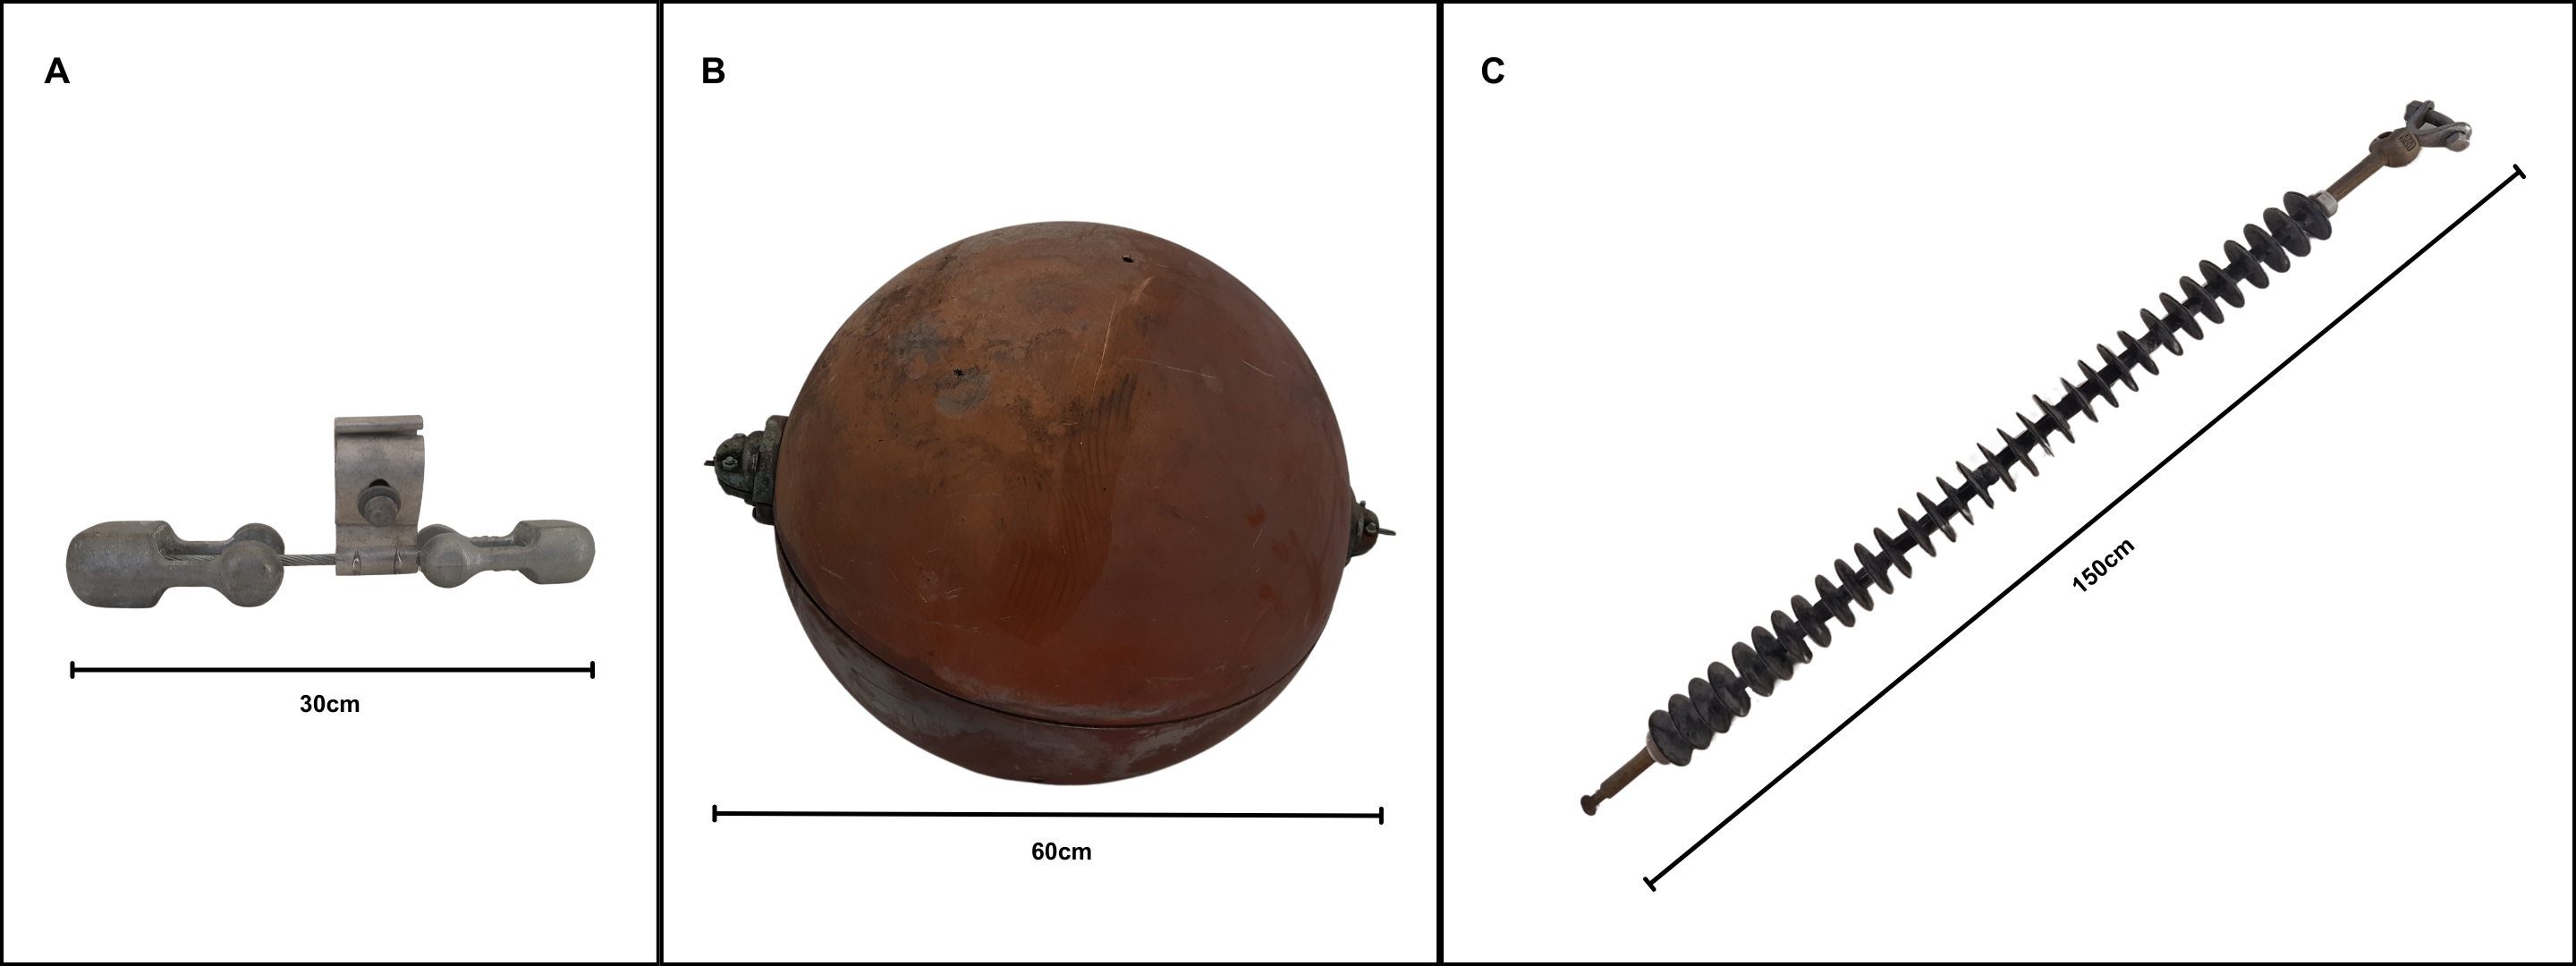
\includegraphics[width=0.8\textwidth]{Objetos.png} 
%     \caption{Objetos a Serem Detectadas}
%     \label{fig:classes_objetos}
% \end{figure}

% \begin{figure}[h]
%         \centering
%         \includegraphics[width=0.8\textwidth]{ObjetosSimu.png} 
%         \caption{Objetos a Serem Detectadas (Simulação)}
%         \label{fig:classes_objetos}
%     \end{figure}

\subsection{Sensores utilizados}

Neste projeto, foram utilizados dois tipos de sensores: o LiDAR e a câmera de profundidade. O LiDAR funciona emitindo feixes de luz laser que são refletidos pelos objetos ao seu redor. A partir do tempo que o feixe leva para retornar ao sensor, é possível calcular a distância até o objeto com alta precisão. Ele gera um valor de distância para cada ângulo de varredura, cobrindo um campo de visão de 360º, o que permite mapear a estrutura tridimensional do ambiente de forma eficiente. Já a câmera de profundidade utiliza luz infravermelha para gerar um mapa denso de profundidade, capturando a distância de cada ponto em sua linha de visão. Diferentemente do LiDAR, que mede distâncias pontuais a partir de um feixe, a câmera de profundidade fornece uma imagem completa com a informação de distância de cada pixel.

\subsection{Planejamento da Coleta de Dados}

A coleta de dados neste trabalho foi planejada com o objetivo de gerar uma base diversificada e representativa de amostras que permitisse o treinamento eficaz de modelos de aprendizado de máquina para a classificação de objetos em linhas de transmissão. Para isso, buscou-se capturar diferentes características espaciais dos objetos de interesse, considerando variações de distância. Foram utilizados dois tipos de sensores de profundidade, de modo a enriquecer a base com diferentes perspectivas e formatos de dados. A coleta foi realizada em dois cenários distintos, um simulado e outro real, seguindo um protocolo padronizado de captura de múltiplas amostras por objeto. Em ambos os cenários, será coletado um total de 150 instâncias de dados para cada tipo de objeto, totalizando um número significativo de amostras que ajudam na robustez do modelo de aprendizado. Cada instância corresponde a uma varredura de 360º realizada pelo LiDAR, bem como uma imagem capturada pela câmera de profundidade, com cada amostra variando em relação à distância do robô aos objetos, e consequentemente, a distância entre os sensores e os mesmos. Os dados foram organizados e rotulados de forma a permitir sua posterior divisão em conjuntos de treinamento, validação e teste. 

A base de dados coletada neste trabalho é crucial para o treinamento dos modelos de aprendizado de máquina, pois sua riqueza em informações determina diretamente a eficácia e precisão da classificação dos objetos. Quanto mais diversificada e representativa for a base de dados, mais robusto e preciso será o modelo treinado, ainda que o treinamento se torne mais intenso e demorado devido ao volume de dados. O objetivo principal da coleta é capturar as características espaciais dos objetos de interesse. Espera-se que os sensores de profundidade possam extrair informações detalhadas sobre a geometria dos objetos, suas dimensões, e suas posições relativas dentro do ambiente de inspeção. Esses dados são essenciais para permitir uma classificação precisa e eficiente dos diferentes tipos de objetos encontrados durante a inspeção das linhas de transmissão.

\subsection{Organização e Formato dos Dados Coletados}

Para possibilitar o uso eficiente dos dados capturados no treinamento e validação dos modelos de aprendizado de máquina, adotou-se uma estrutura de armazenamento clara e padronizada. Os dados do sensor LiDAR foram armazenados em arquivos \textit{CSV} (Comma-Separated Values), e os dados da câmera de profundidade foram salvos em imagens no formato \textit{PNG} (Portable Network Graphics), ambos amplamente compatíveis com bibliotecas de processamento. Além disso, cada amostra foi acompanhada por metadados como rótulo da classe, origem (simulado ou real) e timestamp, assegurando organização e rastreabilidade.

No caso do LiDAR, cada arquivo CSV contém 150 leituras, correspondendo a 150 amostras capturadas em diferentes distâncias entre o robô e o objeto. Cada linha representa uma leitura completa, e cada coluna corresponde a um ângulo fixo dentro do campo de visão de 360°, com os valores expressando distâncias em metros (até 12 m). A estrutura tabular simplifica o processamento e permite fácil inspeção e depuração, além de possibilitar sincronização com os dados da câmera.

As imagens da câmera de profundidade foram salvas em escala de cinza, com codificação ajustada conforme a origem dos dados. Para as imagens obtidas na simulação, os valores de cada pixel foram representados por inteiros sem sinal de 8 bits, totalizando uma escala de 0 a 255. Cada valor nessa escala foi linearmente associado a uma distância entre 0 e 10 metros, permitindo a reconstrução aproximada da profundidade observada em cada ponto da imagem. Já para a câmera real, os valores de pixel foram salvos utilizando inteiros sem sinal de 16 bits, com valores de 0 a 65.535. Nesse caso, a correspondência entre o valor do pixel e a distância é direta: cada unidade representa um milímetro de distância entre o objeto e o sensor. Em ambos os casos, a resolução da câmera foi mantida em 1280 × 720 pixels, garantindo consistência na estrutura dos dados para posterior processamento.

Para assegurar a correta associação entre sensores e objetos, cada leitura foi feita com apenas um objeto presente no campo de visão, o que elimina ambiguidades na rotulagem. Os dados foram organizados em pastas hierárquicas: o diretório principal indica a origem (\textit{real} ou \textit{simulado}) e contém subpastas nomeadas conforme o tipo de objeto (amortecedor, isolador, sinalizador ou nenhum), o que facilita a navegação e o uso por scripts automatizados.

\subsection{Ferramentas e Scripts de Coleta}

A aquisição dos dados foi conduzida por meio de scripts desenvolvidos em Python~\cite{python}, integrados ao ROS para gerenciar a comunicação entre os componentes do sistema. Esses scripts eram responsáveis por subscrever os tópicos dos sensores LiDAR e da câmera de profundidade, controlar o fluxo de aquisição e salvar os dados de forma sincronizada.

Para manipulação e organização dos dados, foram empregadas bibliotecas amplamente utilizadas na comunidade científica. O \textit{NumPy}~\cite{2020NumPy-Array} foi utilizado para processar vetores numéricos com eficiência, enquanto o \textit{Pandas}~\cite{mckinney2010data} facilitou a estruturação e exportação dos dados em arquivos \textit{CSV}. Para as imagens de profundidade, a biblioteca \textit{OpenCV}~\cite{opencv_library} foi utilizada na conversão e salvamento das imagens no formato \textit{PNG} em escala de cinza, conforme os padrões de codificação descritos anteriormente.

A coleta foi automatizada por meio de um loop de captura controlado, no qual cada iteração realizava a aquisição simultânea dos dados dos dois sensores. Entre as capturas, o robô era deslocado progressivamente em direção ao objeto alvo, com a distância de movimentação variando conforme o tipo de objeto analisado. Isso permitiu a obtenção de amostras com diferentes distâncias, aumentando a diversidade e representatividade da base de dados.

Para garantir a integridade e rastreabilidade dos dados, implementou-se também um sistema de registro de logs. Esse sistema armazenava informações como timestamp das amostras, falhas na leitura e inconsistências detectadas. Leituras fora do padrão esperado, como arquivos corrompidos, valores nulos ou discrepantes, foram automaticamente sinalizadas e descartadas.

Essa abordagem automatizada e monitorada proporcionou uma coleta de dados robusta, consistente e reprodutível, minimizando a intervenção manual e otimizando o tempo necessário para aquisição.

\subsection{Pré-processamento Inicial}

Devido ao funcionamento do sensor LiDAR, que realiza leituras em 360°, foi necessário filtrar os dados para considerar apenas os ângulos relevantes ao projeto, uma vez que essa configuração não pode ser alterada diretamente via hardware ou firmware. Assim, durante a captura, são selecionados apenas os valores correspondentes à faixa angular de interesse.

Já as imagens capturadas pela câmera de profundidade não passaram por pré-processamento antes do salvamento, pois os dados foram armazenados diretamente no formato esperado para as etapas subsequentes.

\subsection{Considerações Éticas e Reprodutibilidade}

O processo de coleta de dados foi planejado para garantir que outros pesquisadores possam replicar os experimentos e utilizar a base de dados gerada. Para isso, toda a metodologia, configurações dos sensores, scripts de aquisição e construção dos cenários simulados foram documentados detalhadamente. Além disso, os dados coletados e os datasets construídos estão disponíveis para acesso público no seguinte endereço: \href{https://drive.google.com/drive/folders/15SVMC3oxSVKuzv5S0CRKXIKJzF0k-9lz?usp=sharing}{Datasets}. 

O objetivo é que o projeto seja totalmente replicável, ou que seus dados possam ser reutilizados em trabalhos futuros, mediante solicitação prévia para fins de colaboração ou desenvolvimento.

Quanto à qualidade dos dados, foram aplicados filtros para eliminar valores aberrantes ou muito discrepantes durante as aquisições. As rotulações foram cuidadosamente revisadas para evitar erros de classificação. A quantidade de amostras para cada tipo de objeto é considerada suficiente para o escopo deste trabalho, cobrindo variações realistas de distância entre os sensores e os objetos.

Entretanto, é importante destacar que, apesar dos cuidados adotados, algumas fontes de viés podem estar presentes nos dados. Por exemplo, a coleta realizada em ambientes controlados, tanto simulados quanto reais, pode não contemplar todas as variações e ruídos presentes em situações operacionais reais. Além disso, a escolha dos objetos e das distâncias pode influenciar a representatividade dos dados para outros cenários. Reconhecer essas limitações é fundamental para a correta interpretação dos resultados e para orientar futuros trabalhos de validação e expansão da base.

\section{Construção das Cenas Simuladas}

Nesta seção são apresentados os procedimentos adotados para a criação das cenas simuladas no ambiente virtual, essenciais para a coleta controlada dos dados utilizados no treinamento e validação dos modelos de classificação. A simulação permitiu a definição precisa da configuração espacial dos sensores e dos objetos de interesse, a experimentação ágil de diferentes cenários e parâmetros, além de garantir segurança e redução de custos ao evitar o desgaste e riscos associados à operação em ambientes reais. Os detalhes da modelagem, posicionamento dos sensores, controle do robô simulado e integração com o ROS serão detalhados nas subseções seguintes, assim como o protocolo de coleta e as limitações inerentes ao uso da simulação.

\subsection{Ambiente Virtual Criado no CoppeliaSim}

A estrutura geral da cena simulada consistia em duas torres de transmissão posicionadas a 100 metros de distância uma da outra, conectadas por um cabo cilíndrico e retilíneo, sem curvaturas, a fim de simplificar a análise e evitar instabilidades na simulação. Os objetos de interesse foram pendurados ao longo do cabo, dispostos de forma que pudessem ser capturados individualmente pelos sensores. O robô foi posicionado sobre o cabo com liberdade de movimento linear, controlado pelo usuário por meio de comandos com velocidade ajustável. Os sensores foram acoplados a um suporte fixado no robô, permitindo sua movimentação ao longo da linha.

A modelagem dos componentes utilizados na simulação foi realizada por meio de uma combinação entre o software SolidWorks e os recursos nativos do CoppeliaSim. Os modelos dos robôs foram inicialmente criados no SolidWorks, o que possibilitou uma construção geométrica precisa. Posteriormente, foram exportados para o CoppeliaSim, onde as partes dinâmicas dos robôs foram substituídas por formas primitivas, como cubos e cilindros, a fim de garantir maior leveza e estabilidade na simulação sem comprometer a fidelidade das interações físicas.

Os objetos de interesse para classificação — amortecedores, isoladores e sinalizadores — bem como as torres, também foram modelados no SolidWorks e importados integralmente para o simulador. Diferente do robô, esses elementos mantiveram suas formas completas, pois era essencial preservar suas características físicas e visuais para uma correta detecção e classificação pelos sensores. O cabo foi representado por um cilindro simples, evitando o uso de simulação de curvatura realista, que poderia sobrecarregar o ambiente.

Para assegurar a portabilidade do sensor multimodal (LiDAR e câmera de profundidade) entre diferentes plataformas robóticas, foi desenvolvido um suporte específico no SolidWorks, projetado para manter os sensores corretamente alinhados e fixos. Esse suporte foi integrado ao robô no ambiente do CoppeliaSim, e pode ser facilmente adaptado a diferentes topologias robóticas, permitindo testes variados com o mesmo conjunto de sensores.

A complementaridade dos sensores utilizados está diretamente relacionada à sua posição no robô: a câmera de profundidade foi posicionada na parte superior, oferecendo uma visão panorâmica da porção superior do cabo e dos objetos suspensos, enquanto o LiDAR foi instalado abaixo do robô, capturando dados da região inferior. A combinação dessas perspectivas amplia a qualidade e a riqueza dos dados obtidos, fornecendo uma visão tridimensional mais completa dos componentes inspecionados nas linhas de transmissão.

\subsection{Robô Simulado}

Neste projeto, foram utilizados três protótipos de robôs simulados com o objetivo principal de testar a portabilidade e a adaptabilidade do suporte de sensores entre diferentes topologias robóticas. No entanto, apenas um desses robôs foi utilizado para a coleta dos dados de treinamento dos modelos, enquanto os outros dois serviram para validar o desempenho dos modelos em estruturas distintas.

O robô utilizado na fase de treinamento é o mais simples dos três. Sua estrutura é composta por um suporte de sensores posicionado de forma perpendicular ao cabo e alinhado ao corpo do robô. Ele possui um mecanismo de travamento que permite sua fixação ao cabo e é capaz de realizar deslocamentos lineares com velocidade ajustável, controlada via ROS. A simplicidade desse modelo favorece maior estabilidade durante a coleta de dados, reduzindo variáveis que poderiam interferir nos resultados.

Os dois robôs adicionais apresentam maior complexidade estrutural e foram projetados para superar obstáculos presentes nas linhas de transmissão. Nesses modelos, o suporte dos sensores foi instalado com uma leve inclinação em relação ao corpo principal do robô, simulando diferentes ângulos de visualização. Ambos mantêm o mesmo sistema de controle via ROS, com velocidades lineares também ajustáveis por código, permitindo comparações consistentes com o modelo mais simples.

A construção dos sistemas robóticos foi inteiramente baseada em juntas rotacionais simples disponibilizadas pelo CoppeliaSim. Essas juntas simulam movimentos giratórios básicos e, quando combinadas, possibilitam a reprodução de movimentos mais complexos. Todas as juntas foram integradas ao ROS, o que facilitou a implementação e o controle. Essa abordagem modular e padronizada simplifica o desenvolvimento e a replicação do sistema em diferentes configurações robóticas.

\subsection{Integração com ROS}

A integração entre o ambiente de simulação CoppeliaSim e o sistema ROS foi realizada por meio de scripts escritos em Lua diretamente no simulador. Cada objeto da cena recebe um identificador único no script, o que permite controlar suas propriedades diretamente. No caso de juntas, por exemplo, é possível configurar parâmetros como torque e velocidade.

Utilizando a biblioteca integrada do ROS fornecida pelo CoppeliaSim, foram implementados publicadores e assinantes diretamente nos scripts em Lua. Essa comunicação permite que o simulador interaja em tempo real com o ROS rodando na máquina. As juntas do robô foram controladas por assinantes que recebiam comandos externos, gerados por um código fora do ambiente CoppeliaSim, sob controle do usuário. Por outro lado, os sensores, como a câmera de profundidade e o LiDAR, funcionaram como publicadores, transmitindo dados para seus respectivos tópicos definidos no script de simulação. Esses dados eram então capturados por outro código externo responsável por processá-los e armazená-los para uso posterior.

Para garantir a confiabilidade da integração e dos dados utilizados nos experimentos, foram realizados testes de validação. Objetos foram posicionados a distâncias conhecidas dos sensores, permitindo verificar a acurácia dos dados de profundidade publicados. Além disso, foi verificada a sincronização temporal e espacial entre os sensores antes do início da coleta definitiva dos dados, assegurando que as leituras fossem consistentes e alinhadas para uso no treinamento dos modelos de classificação.

\subsection{Protocolo de Coleta na Simulação}

Para realizar a coleta de dados nas cenas simuladas, os objetos foram posicionados individualmente à frente dos sensores do robô. O controle do robô foi feito manualmente pelo usuário, que o aproximava dos objetos até que o sensor LiDAR detectasse sua presença. A partir desse momento, era iniciada a gravação dos dados, enquanto o robô se deslocava em direção ao objeto com velocidade constante.

A velocidade de deslocamento foi configurada de forma distinta para cada objeto, levando em consideração suas dimensões. Objetos menores, por exemplo, exigiram velocidades menores para garantir uma quantidade suficiente de amostras, de modo a equilibrar o volume de dados coletado em relação aos objetos maiores.

Após a coleta, os dados passaram por um processo de inspeção para a identificação e remoção de valores discrepantes ou incoerentes. Caso necessário, o processo de aquisição era repetido, a fim de garantir que os dados representassem com fidelidade o objeto analisado. Os dados finais foram então organizados e armazenados de maneira estruturada, incluindo os rótulos correspondentes a cada classe de objeto, para posterior uso no treinamento e avaliação dos modelos de aprendizado de máquina.

\subsection{Limitações e Considerações sobre a Simulação}

A simulação apresenta algumas limitações em relação ao ambiente real, principalmente no que diz respeito à fidelidade das leituras dos sensores. Nos ambientes simulados não há presença de ruídos, reflexos ou deformações nos dados capturados, o que favorece a obtenção de informações limpas e consistentes. No entanto, essa ausência de imperfeições pode comprometer a generalização dos modelos treinados exclusivamente com dados simulados, uma vez que sensores reais estão sujeitos a reflexos, interferências e variações físicas nas medições.

Como ambos os sensores utilizados operam por meio da emissão de feixes de luz (infravermelho), o fator que mais impacta a qualidade das medições no mundo real são as reflexões em superfícies irregulares ou brilhantes. Essa característica não é reproduzida na simulação, pois o CoppeliaSim não modela o comportamento real dos feixes de luz nem as propriedades ópticas dos materiais simulados.

Apesar dessas limitações, a simulação desempenha um papel fundamental como etapa preliminar do desenvolvimento. Ela permite gerar conjuntos de dados organizados, com classes bem definidas e isentas de ruído, que são extremamente úteis para a validação inicial dos modelos de aprendizado de máquina. Além disso, os resultados obtidos com dados simulados servem como base de comparação para os modelos treinados com dados reais, oferecendo uma referência inicial sobre o desempenho esperado e facilitando a análise das discrepâncias entre os dois contextos.

\section{Construção das Cenas no Laboratório}

Após a etapa de simulação, torna-se essencial validar o desempenho do sistema em condições reais, onde as limitações dos sensores e os desafios do ambiente físico podem impactar diretamente a eficácia dos modelos desenvolvidos. Esta seção descreve o processo de construção das cenas no laboratório, utilizado como ambiente de testes controlado para replicar, em escala reduzida, os elementos principais de uma linha de transmissão de energia. O objetivo é analisar a robustez do sistema diante de variações naturais e ruídos típicos dos sensores reais, bem como avaliar a viabilidade prática da solução proposta. Serão abordadas desde a infraestrutura física do laboratório, passando pela montagem do protótipo e do cabo suspenso, até os métodos de coleta e gerenciamento dos dados em ambiente real. A integração com o ROS, a comunicação embarcada e a adaptação dos scripts desenvolvidos na simulação para a coleta física também são discutidas, permitindo uma comparação direta entre os dados simulados e reais.


\subsection{Objetivos da Validação em Ambiente Real}

A validação em ambiente real tem como principal finalidade confirmar a viabilidade prática do sistema desenvolvido, observando o comportamento dos sensores físicos e do robô em condições controladas, porém reais. Por meio desses testes, é possível identificar limitações operacionais dos sensores, como perdas de dados por reflexões, ruídos de leitura e falhas na aquisição, que não estão presentes na simulação. Além disso, essa etapa permite avaliar a robustez dos modelos de classificação quando expostos a variações naturais no ambiente, garantindo que o desempenho observado virtualmente possa ser replicado, ao menos em parte, no cenário físico. A coleta em laboratório representa, portanto, um elo essencial entre o ambiente idealizado da simulação e as futuras aplicações operacionais do sistema em campo.

\subsection{Infraestrutura do Laboratório}

Os testes em ambiente real foram realizados em um laboratório com infraestrutura necessária para a montagem de uma linha de transmissão em escala reduzida, bem como para a construção e operação dos protótipos robóticos utilizados no projeto. O espaço físico disponível permitia a instalação de um cabo suspenso com cerca de 5 metros de comprimento, fixado a aproximadamente 2 metros do solo, proporcionando um ambiente controlado e representativo para a realização dos experimentos.

A sustentação do cabo foi viabilizada por meio de suportes metálicos do tipo cotovelo, fixados diretamente às paredes laterais do laboratório. O cabo foi preso aos suportes utilizando abraçadeiras de aço, garantindo rigidez e leve afundamento central, simulando a curvatura natural de cabos em linhas reais. Essa configuração permitiu a instalação segura dos objetos de interesse e possibilitou o deslocamento contínuo do robô ao longo do trecho durante as coletas.

\subsection{Coleta com Robô em Cabo Suspenso}

O robô utilizado nas coletas em ambiente real é uma réplica funcional do modelo empregado nas simulações virtuais. Trata-se de um protótipo móvel desenvolvido para se deslocar linearmente sobre um cabo suspenso, com capacidade de ajuste de velocidade e mecanismos de travamento e destravamento, garantindo segurança e estabilidade durante a movimentação e a aquisição dos dados.

O sistema de locomoção é composto por dois motores de passo: um responsável pelo deslocamento linear ao longo do cabo e outro dedicado ao acionamento do mecanismo de travamento. Ambos os motores são controlados por um microcontrolador Arduino, que atua como interface entre o hardware e o ROS, permitindo a reutilização do mesmo código e lógica de controle aplicados na simulação. A estrutura completa do robô e seu funcionamento detalhado podem ser consultados em \citeonline{10.1007/978-3-031-58676-7_42}.

O controle e a alimentação do sistema são realizados por uma Raspberry Pi 5, que se comunica com o Arduino e com os sensores (LiDAR e câmera de profundidade) por meio de interfaces seriais. Toda a alimentação elétrica é provida por baterias embarcadas, tornando o sistema completamente autônomo e dispensando conexões externas durante os testes.

\subsubsection{Estrutura do cabo suspenso}

A estrutura do experimento consiste em um cabo de alumínio com alma de aço (ACSR — Aluminium Conductor Steel Reinforced), similar aos utilizados em linhas de transmissão reais. O cabo, com cerca de 5 metros de comprimento, foi suspenso a uma altura aproximada de 2 metros do solo, fixado nas extremidades por meio de suportes metálicos do tipo cotovelo ancorados nas paredes do laboratório. A fixação foi feita com abraçadeiras de aço, garantindo estabilidade e uma leve curvatura natural do cabo.

Os objetos de interesse — como isoladores, amortecedores e sinalizadores — foram fixados ao cabo individualmente durante os testes. Os componentes utilizados são peças reais, idênticas às aplicadas em linhas de transmissão de alta tensão, e foram montados utilizando os mesmos métodos de fixação empregados em campo, assegurando uma representação fidedigna do ambiente operacional.

\subsection{Integração com ROS}

Para a integração dos sensores e atuadores no ambiente real, o ROS é executado diretamente na Raspberry Pi 5 embarcada no robô. A Raspberry atuou como nó mestre, sendo responsável pela orquestração e processamento de todas as informações do sistema. No entanto, ela não possui suporte nativo aos sistemas operacionais Ubuntu 20.04 ou Debian 10, os quais são requisitos para o ROS Noetic — versão escolhida para este projeto. Para contornar essa limitação, optou-se pelo uso do Docker, uma plataforma de virtualização leve baseada em contêineres que permite a execução isolada de aplicações em qualquer sistema operacional compatível~\cite{merkel2014docker}.

O contêiner Docker foi configurado com permissões equivalentes ao usuário root do sistema, garantindo acesso irrestrito a portas seriais e arquivos do dispositivo. Dentro desse contêiner, o ambiente ROS foi completamente configurado, incluindo os nós responsáveis por publicar os dados dos sensores e comandar os motores.

O controle dos motores foi realizado por meio do pacote \textit{rosserial}, que provê uma interface de comunicação entre dispositivos embarcados, como o Arduino, e o ROS, permitindo a publicação e subscrição de tópicos por meio de uma conexão serial~\cite{rosserial}.

Para a câmera de profundidade fui utilizada a Intel RealSense D415 com o pacote \textit{realsense-ros}, fornecido pela própria Intel. Esse pacote oferece \textit{launch files} e configurações prontas para a integração da câmera ao ROS, facilitando a captura e publicação dos dados de profundidade e cor~\cite{realsense_ros}.

O sensor LiDAR empregado foi o RPLIDAR A1, cuja integração foi realizada por meio do pacote \textit{rplidar\_ros}, disponibilizado pela Slamtec. O pacote contém arquivos de configuração específicos para cada modelo de sensor, incluindo parâmetros de calibração e tópicos de publicação compatíveis com o ROS~\cite{rplidar_ros}.

Com esses pacotes devidamente configurados e em execução no contêiner Docker, os dados brutos dos sensores passaram a ser publicados em tópicos ROS, estando assim disponíveis para subscrição e processamento por outros módulos do sistema.

A coleta dos dados foi realizada utilizando os mesmos scripts empregados na fase de simulação, garantindo consistência e sincronização entre os sensores. Os dados adquiridos foram armazenados localmente na Raspberry Pi durante as sessões de coleta e, posteriormente, transferidos para uma estação de trabalho dedicada, onde foram utilizados para o treinamento e validação dos modelos de classificação.

\subsection{Protocolo de Coleta no Laboratório}

A coleta de dados no ambiente real foi conduzida de forma similar à realizada na simulação. O robô foi posicionado de forma manual próximo a cada objeto até que se confirmasse a correta detecção e leitura pelos sensores. Em seguida, o robô foi configurado para se deslocar com velocidade constante ao longo do cabo, realizando a captura dos dados sensoriais.

Cada objeto foi analisado individualmente, sendo necessário ajustar a velocidade do robô para cada caso, de modo a garantir a qualidade da leitura — assim como foi feito na fase de simulação. A velocidade foi escolhida de forma que os sensores pudessem capturar uma quantidade suficiente de amostras com o objeto dentro do campo de visão.

Após a coleta, os dados foram inspecionados manualmente para remoção de valores discrepantes ou amostras com ruídos excessivos. Esse processo garantiu que o conjunto final fosse conciso, representativo e estivesse devidamente rotulado, assegurando a integridade e a confiabilidade das informações utilizadas no treinamento e validação dos modelos de aprendizado de máquina.

\subsection{Comparação com a Simulação}

Os dados coletados com os sensores reais apresentaram níveis de ruído, como era esperado, mas de forma geral mantiveram boa qualidade quando comparados aos dados da simulação, especialmente na análise de objetos com superfícies não reflexivas. Nesses casos, as leituras do LiDAR e da câmera de profundidade se mostraram consistentes e compatíveis com os dados simulados, validando a fidelidade do ambiente de simulação.

No entanto, ao lidar com objetos reflexivos, como o próprio cabo utilizado na estrutura, foram observadas distorções nas leituras. O LiDAR apresentou, em diversos momentos, medições no limite superior de alcance (cerca de 12 metros), especialmente nas primeiras e últimas amostras do objeto, quando os feixes eram emitidos em ângulos muito abertos em relação ao cabo. Tais valores são fisicamente impossíveis dentro do ambiente de teste — cujo teto estava a apenas 2 metros de altura — e indicam perda de dados devido à reflexão inadequada do feixe do sensor.

Já a câmera de profundidade demonstrou dificuldades ainda maiores nesse cenário. Durante toda a coleta, não foi possível obter leituras válidas de profundidade referentes ao cabo, mesmo em posições mais próximas. O sensor simplesmente atribuía o valor zero para esses pontos, indicando que a luz infravermelha não estava sendo refletida de forma adequada para que a profundidade pudesse ser estimada.

\section{Registro e Gestão dos Dados}

A organização dos arquivos gerados seguiu um padrão simples e funcional, dado que os dados foram coletados individualmente para cada objeto e devidamente rotulados no momento da aquisição. Isso evitou a necessidade de processos posteriores de separação ou balanceamento dos dados.

A nomenclatura adotada para os arquivos refletia diretamente o conteúdo dos dados, indicando o nome do objeto, o sensor utilizado (LiDAR ou câmera de profundidade) e a origem dos dados (simulação ou ambiente real). Essa padronização facilitou o processo de criação e manipulação dos \textit{datasets}.

Os dados utilizados para o treinamento dos modelos foram organizados em 10 \textit{datasets} distintos. As divisões foram feitas considerando:

\begin{itemize}
  \item Origem dos dados: simulado ou real;
  \item Tipo de sensor: apenas LiDAR, apenas câmera de profundidade ou ambos combinados;
  \item Forma de representação: dados brutos ou extração de \textit{features}.
\end{itemize}

Cada \textit{dataset} era composto por arquivos no formato \texttt{.csv}, contendo 150 amostras para cada uma das quatro classes de objetos (amortecedor, isolador, sinalizador, nada), totalizando 600 amostras por \textit{dataset}.

Além dos arquivos tabulares, foram criados dois \textit{datasets} adicionais com imagens de profundidade:

\begin{itemize}
  \item Um composto por imagens simuladas, obtidas diretamente do ambiente virtual;
  \item Outro composto por imagens reais, submetidas a técnicas de pré-processamento para remoção de ruído e aprimoramento da qualidade.
\end{itemize}

Esses conjuntos de imagens foram utilizados para o treinamento de uma rede neural convolucional, que serviu como \textit{benchmark} para avaliar a utilidade das informações visuais nas tarefas de classificação.


\section{Treinamento e Avaliação dos Modelos}

Esta seção descreve o processo de modelagem e avaliação dos algoritmos de aprendizado de máquina utilizados para a classificação de objetos em linhas de transmissão, com base em informações de profundidade coletadas por sensores. A motivação para o uso de técnicas de inteligência artificial neste contexto está na capacidade dessas abordagens de extrair padrões complexos dos dados, superando limitações de sistemas baseados apenas em regras ou análise manual. Ao treinar modelos supervisionados com os dados previamente rotulados, busca-se criar um sistema autônomo de classificação que seja robusto a variações dentro de um cenário real ou simulado.

\subsection{Objetivo da Etapa de Treinamento}

A etapa de treinamento tem como propósito utilizar os dados coletados — tanto simulados quanto reais — para desenvolver modelos capazes de classificar automaticamente os objetos encontrados ao longo de uma linha de transmissão, como isoladores, sinalizadores, amortecedores ou a ausência de objetos (classe “nada”). A modelagem visa permitir que, a partir das informações de profundidade fornecidas pelos sensores, seja possível inferir corretamente a classe do objeto observado.

\subsection{Arquiteturas e Algoritmos Testados}

Os modelos testados neste trabalho foram k-Vizinhos Mais Próximos (k-NN), Árvore de Decisão, Naive Bayes, Floresta Aleatória, Perceptron Multicamadas (MLP) e uma Rede Neural Convolucional (SqueezeNet), todos amplamente utilizados em tarefas de classificação. A seguir, descrevemos o funcionamento de cada modelo e seus principais hiperparâmetros, que impactam diretamente o desempenho e a capacidade de generalização. Para uma explicação mais aprofundada, consulte \cite{bishop2006pattern}.

\subsubsection{k-Vizinhos mais proximos}

O kNN é um modelo de aprendizado supervisionado que classifica um objeto com base na proximidade com exemplos já conhecidos no espaço de características. O princípio básico é encontrar os \textit{k} exemplos mais próximos (vizinhos) e decidir a classe do novo objeto segundo as classes desses vizinhos.

Os hiperparâmetros importantes do kNN incluem o número de vizinhos considerados, que define quantos exemplos próximos serão usados para a decisão, a métrica de distância, que determina como a proximidade entre pontos é calculada e pode influenciar a sensibilidade do modelo a diferentes características, e o esquema de pesos, que pode dar maior importância a vizinhos mais próximos.

\subsubsection{Árvore de Decisões}

A árvore de decisões utiliza uma estrutura hierárquica de perguntas sobre atributos dos dados para chegar a uma classificação final. Cada nó interno representa uma condição sobre um atributo e as folhas indicam a classe predita.

Os hiperparâmetros que controlam a árvore incluem a profundidade máxima, que limita o tamanho da árvore para evitar que ela se ajuste demais aos dados de treinamento (\textit{overfitting}), o número mínimo de amostras para dividir um nó, e o número mínimo de amostras para formar uma folha. Esses parâmetros ajudam a balancear a complexidade do modelo.

\subsubsection{Naive Bayes}

O Naive Bayes é um modelo probabilístico que assume independência condicional entre as características dado a classe. Ele calcula a probabilidade de cada classe dado o vetor de características e escolhe a mais provável.

Embora possua poucos hiperparâmetros, um deles é a escolha da distribuição probabilística usada para modelar os dados, como Gaussiana ou multinomial, o que afeta o cálculo das probabilidades condicionais e, consequentemente, o desempenho do modelo.

\subsubsection{Floresta Aleatória}

A Floresta Aleatória é um conjunto de árvores de decisão treinadas em subconjuntos aleatórios dos dados e características, cuja decisão final é feita por votação entre as árvores.

Os principais hiperparâmetros são o número de árvores no conjunto, que influencia a estabilidade e robustez da predição; a profundidade máxima das árvores; o número mínimo de amostras para dividir nós ou formar folhas; e o número máximo de características consideradas em cada divisão, que impacta a diversidade entre as árvores e ajuda a evitar \textit{overfitting}.

\subsubsection{Perceptron Multicamadas}

O MLP é uma rede neural feedforward composta por múltiplas camadas de neurônios totalmente conectados, capaz de modelar relações não lineares complexas entre as características e as classes.

Seus hiperparâmetros incluem a arquitetura da rede, ou seja, o número de camadas e neurônios por camada, que definem a capacidade de representação do modelo; a taxa de aprendizado, que afeta a velocidade e qualidade da convergência durante o treinamento; a função de ativação, que introduz não linearidade; e o número de épocas, que determina quantas vezes o conjunto de dados é usado para atualizar os pesos.

\subsubsection{Rede Neural Convolucional – SqueezeNet}

Além dos modelos clássicos, foi utilizada uma rede neural convolucional para classificação das imagens de profundidade capturadas pela câmera. A rede escolhida foi a SqueezeNet \cite{SqueezeNet}, que é conhecida por atingir acurácia comparável à AlexNet com um número muito menor de parâmetros e tamanho reduzido do modelo, facilitando sua implementação em sistemas embarcados.

A SqueezeNet é composta por blocos “fire”, que combinam camadas convolucionais de filtros pequenos (1x1) e maiores (3x3) para extrair características complexas das imagens de forma eficiente. Seus hiperparâmetros envolvem a configuração do número de filtros em cada camada, o tamanho dos filtros convolucionais, além dos parâmetros típicos de treinamento, como taxa de aprendizado, tamanho do lote (batch size) e número de épocas. Esperava-se que essa rede apresentasse desempenho superior em acurácia, ainda que com tempo de processamento maior que os modelos clássicos, sendo usada como referência para validação dos dados obtidos pela câmera de profundidade.

\subsection{Treinamento dos Modelos}

Os modelos foram treinados utilizando ferramentas robustas e amplamente adotadas na comunidade de aprendizado de máquina e aprendizado profundo. As principais bibliotecas utilizadas foram o \texttt{scikit-learn} e o \texttt{PyTorch}, ambas desenvolvidas em Python.

O \texttt{scikit-learn} é uma biblioteca de aprendizado de máquina de alto nível que oferece uma ampla variedade de algoritmos clássicos, incluindo kNN, árvores de decisão, Naive Bayes e Florestas Aleatórias, além de utilitários para pré-processamento, avaliação e seleção de modelos. Sua interface simples e eficiente facilita a implementação rápida de experimentos, sendo ideal para o treinamento e validação dos modelos clássicos usados neste trabalho \cite{pedregosa2011scikit}.

Já o \texttt{PyTorch} é uma biblioteca focada em aprendizado profundo, que proporciona um estilo imperativo de programação com alta performance e flexibilidade na construção de redes neurais, como a rede convolucional SqueezeNet utilizada neste projeto. Com suporte dinâmico para computação em GPU e funcionalidades avançadas para otimização e manipulação de tensores, o PyTorch permite o desenvolvimento e treinamento eficiente de modelos complexos \cite{NEURIPS2019_9015}.

Essas ferramentas complementares permitiram o desenvolvimento dos modelos clássicos e da rede neural convolucional, garantindo uma base sólida para o processo de treinamento e avaliação.

\subsection{Avaliação de Desempenho}

A avaliação dos modelos desenvolvidos foi realizada utilizando a técnica de validação cruzada, que consiste em dividir o conjunto de dados em subconjuntos para garantir uma análise mais robusta e menos enviesada do desempenho do modelo. Na validação cruzada, os dados são segmentados em múltiplas partições, onde, em cada iteração, um subconjunto é utilizado para teste enquanto os demais servem para treinamento. Esse processo é repetido até que todos os subconjuntos tenham sido usados como teste, e os resultados são então agregados para obter uma estimativa geral da performance.

A métrica escolhida para quantificar o desempenho dos modelos foi a acurácia, definida como a proporção de classificações corretas em relação ao total de amostras avaliadas. A acurácia é uma medida intuitiva e amplamente utilizada para problemas de classificação, pois indica diretamente a eficácia do modelo em reconhecer corretamente as classes presentes nos dados.

Além da avaliação tradicional, foi realizada uma validação específica para testar a capacidade dos modelos de generalizar entre diferentes configurações robóticas. Para isso, os modelos foram treinados utilizando um dataset obtido a partir de uma topologia robótica e validados em outro conjunto de dados capturado por uma topologia distinta. Essa abordagem visa avaliar a robustez do sistema frente a variações nas topologias de robôs inspetores.

O tempo gasto no processo de validação foi também monitorado, pois é um fator importante para aplicações em sistemas embarcados e em tempo real, onde a eficiência computacional é crítica para o funcionamento prático dos classificadores.

\subsection{Limitações da Metodologia}

A metodologia adotada neste trabalho apresenta algumas limitações importantes, principalmente relacionadas à coleta de dados reais para treinamento e validação dos modelos. Primeiramente, a coleta de dados reais está sujeita a restrições de espaço físico disponível no laboratório. O que impacta diretamente na representatividade e diversidade dos dados coletados.

No ambiente simulado, apesar de fornecer uma boa aproximação do cenário real de uma linha de transmissão, os sensores não sofrem interferências externas, como ruídos e reflexões, o que resulta em dados mais limpos e idealizados, que podem não refletir completamente as condições reais encontradas em campo.

Por outro lado, no ambiente de laboratório, os dados são capturados de sensores reais e, portanto, incluem reflexões e interferências típicas do mundo real, tornando-os mais concretos. Contudo, devido ao espaço físico limitado, o cenário representa apenas uma aproximação parcial das condições reais de uma linha de transmissão. Especificamente, o fundo de escala dos sensores nesse ambiente varia entre 2 e 5 metros, enquanto em uma estrutura real o fundo de escala pode alcançar até 12 metros, devido à ausência de objetos além da própria linha. Isso implica que as leituras obtidas no laboratório não reproduzem com fidelidade todas as características do ambiente real.

Além disso, por se tratar de um ambiente controlado, existe o risco de \textit{overfitting} dos modelos, isto é, os modelos podem apresentar bom desempenho nos dados utilizados para treinamento, mas ter baixa capacidade de generalização para situações não contempladas, como a presença de objetos inesperados na linha de transmissão ou variações significativas na posição dos objetos.

Essas limitações indicam a necessidade de futuras coletas de dados em ambientes reais e diversificados para melhorar a robustez e aplicabilidade dos modelos desenvolvidos.




%-----------------------------------------------------------%